\documentclass{beamer}
\usepackage{color} 
\usepackage{}  
\usepackage{hyperref}
\hypersetup{
	colorlinks=true, 
	linktoc=all,     
	linkcolor=blue,  
	allcolors=blue
}
\graphicspath{ {../images/} }
\title[Seminar presentation] %optional
{Shape formation using Kilobots}
\subtitle{A finite state machine approach}
 
\author[shortname]{Kishan\inst{1} \and Eswara Srisai\inst{1} \and Sudhakar\inst{1} \and Anurag\inst{1}}

 
\institute[VFU] % (optional)
{
  \inst{1}%
  M.Tech scholar\\
  Systems and Control Engineering
}

\date[VLC 2013] % (optional)
{\href{http://www.iitb.ac.in/}{Indian Institute of Technology, Bombay}\\\today}
\begin{document}
\setlength\abovecaptionskip{-2pt}	
\setlength{\abovedisplayskip}{0pt}
\setlength{\belowdisplayskip}{0pt}
\setlength{\abovedisplayshortskip}{0pt}
\setlength{\belowdisplayshortskip}{0pt}
\AtBeginSection[]
{
	\begin{frame}<beamer>
	\frametitle{Overview}
	\tableofcontents[currentsection]
	\end{frame}
}

\frame{\titlepage}

\begin{frame}
	\frametitle{About Kilobots}
	\begin{columns}
		\begin{column}{0.4\textwidth}
			\begin{figure}
				\centering
				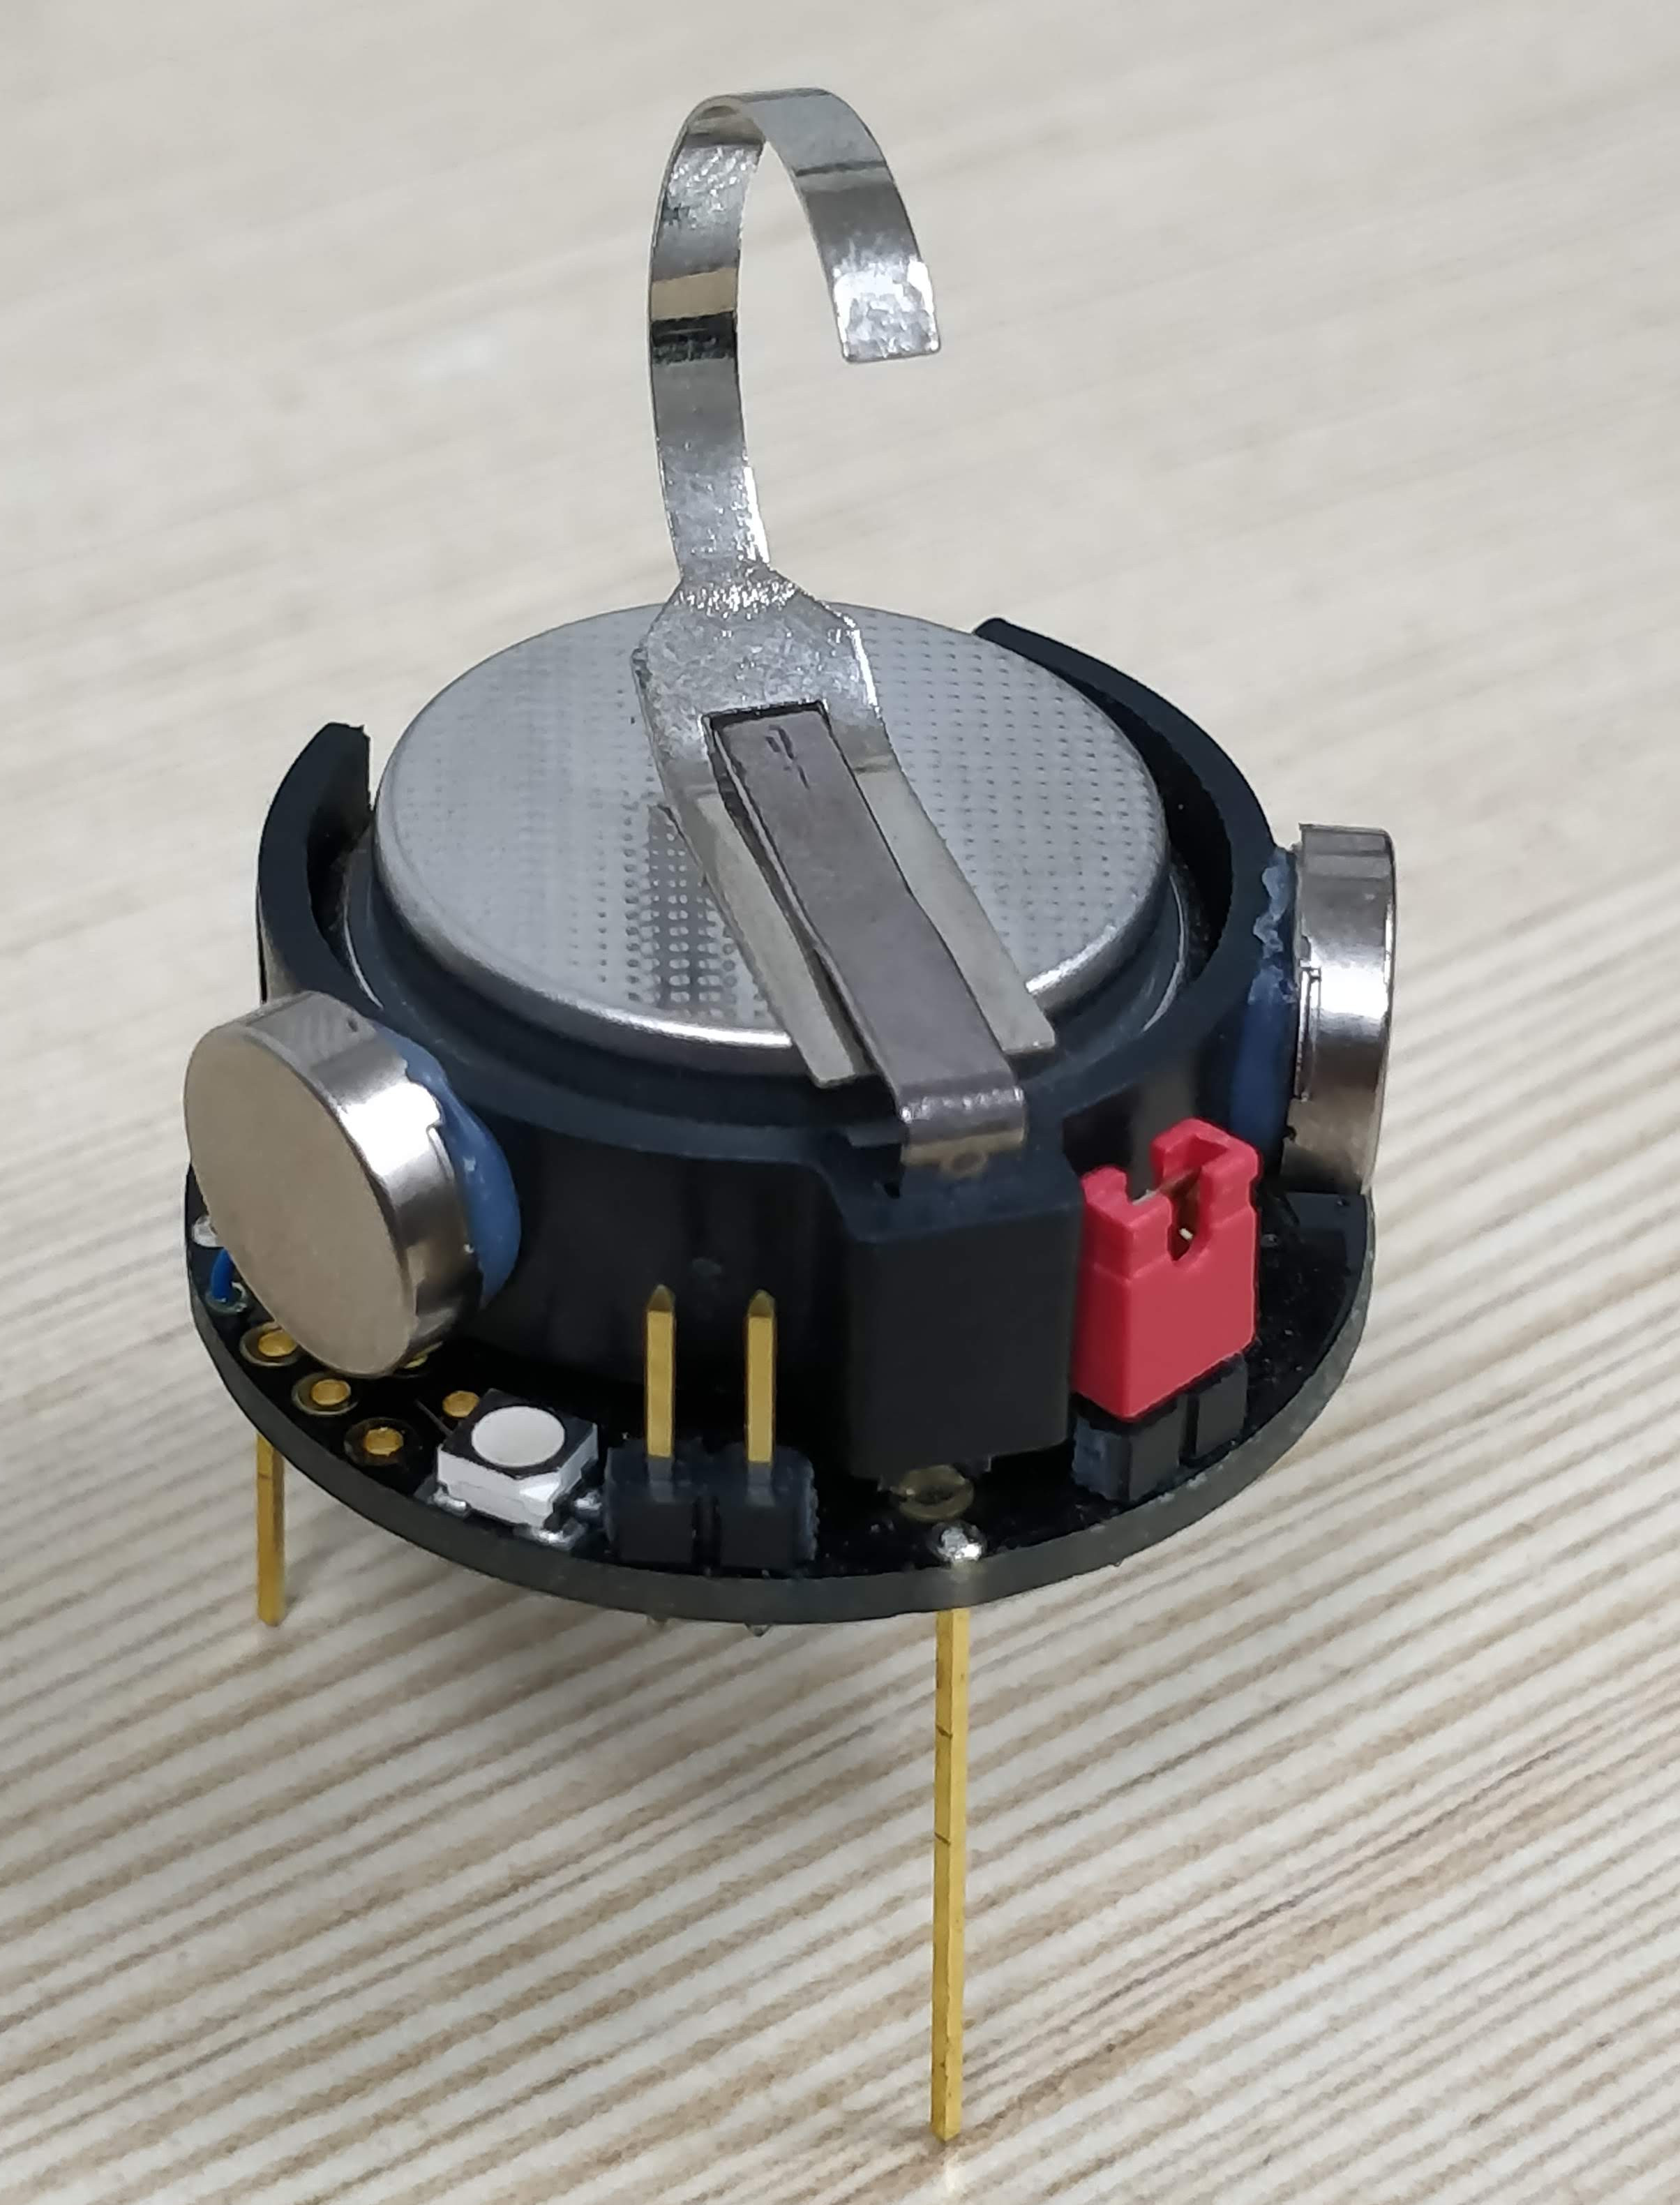
\includegraphics[scale=0.05]{kilobots}
				\caption{Kilobot}
			\end{figure}
		\end{column}
						
		\begin{column}{0.45\textwidth}
			\begin{itemize}
				\item ATmega 328p processor 
				\item Li-Ion 3.7V battery 
				\item IR sensor 
				\item Light sensor 
				\item Vibration motors (1 cm/sec, 45 degrees/sec)
			\end{itemize}
		\end{column}
	\end{columns}
\end{frame}

\begin{frame}
	\frametitle{About Kilobots}
	\begin{columns}
		\begin{column}{0.4\textwidth}
			\begin{figure}
				\centering
				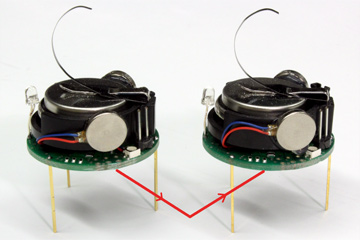
\includegraphics[scale=0.4]{comm}
				\caption{Communication between two Kilobots}
			\end{figure}
		\end{column}
						
		\begin{column}{0.45\textwidth}
			\begin{itemize}
				\item Reflecting IR light
				\item Communication up to 7 cm (32kb/s) away 
				\item Using over-head controller
			\end{itemize}
		\end{column}
	\end{columns}
\end{frame}

\begin{frame}
	\frametitle{Channel use by Kilobots}
	\begin{itemize}
		\item Sharing of same wireless channel by all robots
		\item CSMA-CA (Carrier Sense Multiple Access with Collision Avoidance) method 
		\item Reduction of channel bandwidth        
	\end{itemize}
\end{frame}

\begin{frame}
	\frametitle{About Kilobots}
	\begin{columns}
		\begin{column}{0.4\textwidth}
			\begin{figure}
				\centering
				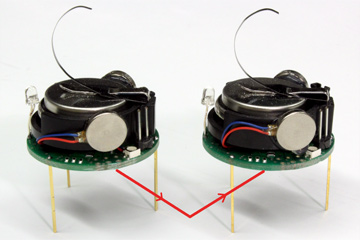
\includegraphics[scale=0.4]{comm}
				\caption{Communication between two Kilobots}
			\end{figure}
		\end{column}
		
		\begin{column}{0.45\textwidth}
			\begin{itemize}
				\item Reflecting IR light
				\item Communication up to 7 cm away 
				\item Using over-head controller
			\end{itemize}
		\end{column}
	\end{columns}
\end{frame}

\begin{frame}
\only<1-2>{
	\frametitle{Efficient orbiting using a Finite State Machine (FSM)}
	\only<1->{
		\textbf{Objective:} Algorithm to allow a planet to orbit n stars from any initial condition.
	}
	\begin{itemize}
		\only<1->{
			\item \textbf{Stars:} Stationary bots around which planet rotates (Black)
			\item \textbf{Planet:} Dynamic bots rotating around stars (Gray)
		}
	\end{itemize}
			\begin{columns}
			\begin{column}{0.2\textwidth}
				\begin{figure}
					\centering
					\only<1>
					{
					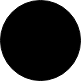
\includegraphics[scale=0.25]{star1}
					}
					\only<2>
					{
						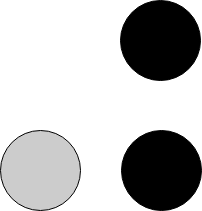
\includegraphics[scale=0.25]{star2planet}
					}
					\hspace{5 cm}
					\caption{Single star system}
				\end{figure}
			\end{column}
			\begin{column}{0.33\textwidth}	
				\begin{figure}
					\centering
					\only<1>
					{
						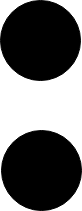
\includegraphics[scale=0.25]{star2}
					}
					\only<2>
					{
						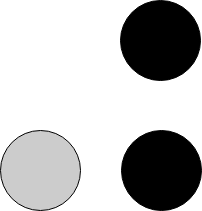
\includegraphics[scale=0.25]{star2planet}
					}
					\hspace{5 cm}
					\caption{Linear star system}
				\end{figure}
			\end{column}
			\begin{column}{0.33\textwidth}
				\begin{figure}
					\centering
					\only<1>
					{
						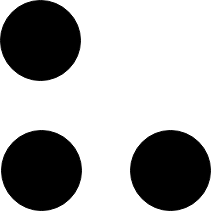
\includegraphics[scale=0.25]{star3}
					}
					\only<2>
					{
						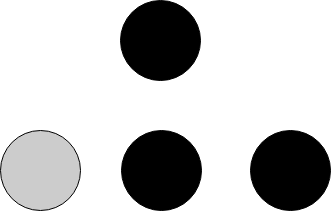
\includegraphics[scale=0.25]{star3planet}
					}
					\hspace{5 cm}
					\caption{Triangular star system}
				\end{figure}
		\end{column}
	\end{columns}
}
\end{frame}
\begin{frame}
\frametitle{\small Flowchart}
\begin{figure}[H]
	\centering
	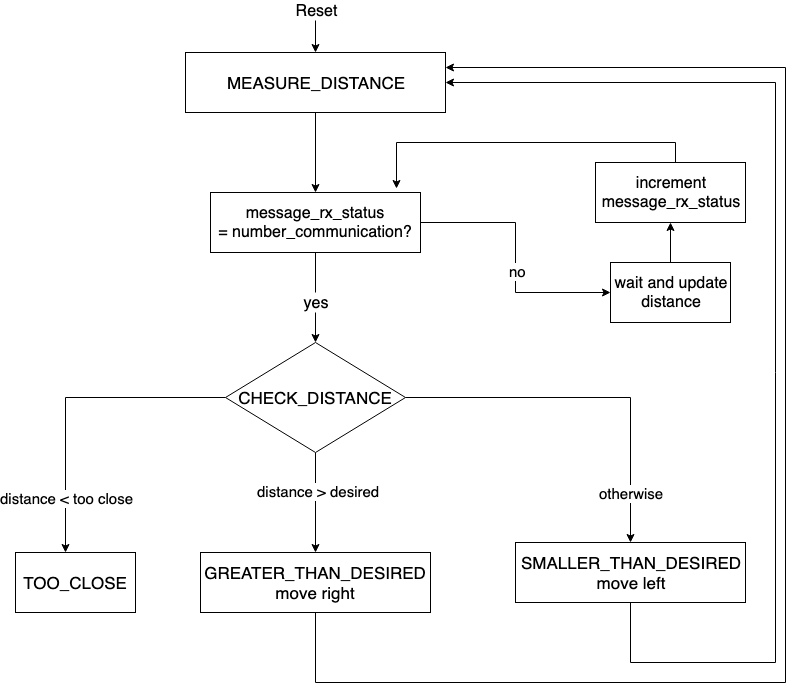
\includegraphics[scale=0.3]{star_planet_escape1}
	\caption{Flowchart for shape formation algorithm}
	\label{fig:fc_shape_form}
\end{figure}
\end{frame}
\begin{frame}
\frametitle{\small Flowchart}
\begin{figure}[H]
	\centering
	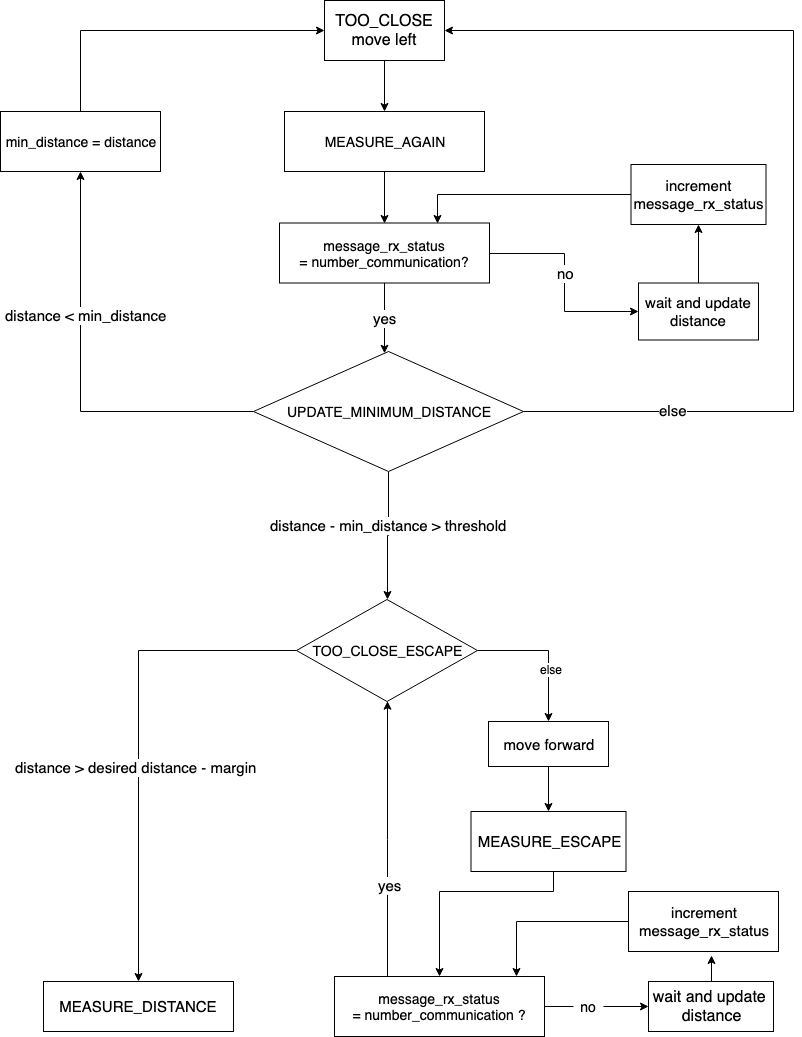
\includegraphics[scale=0.2]{star_planet_escape2}
	\caption{Flowchart for shape formation algorithm}
	\label{fig:fc_shape_form}
\end{figure}
\end{frame}
\begin{frame}
	\frametitle{Shape formation}
	\framesubtitle{Demonstration}
	\begin{columns}
	\begin{column}{0.5\textwidth}
	\begin{figure}[H]
		\centering
		\fbox{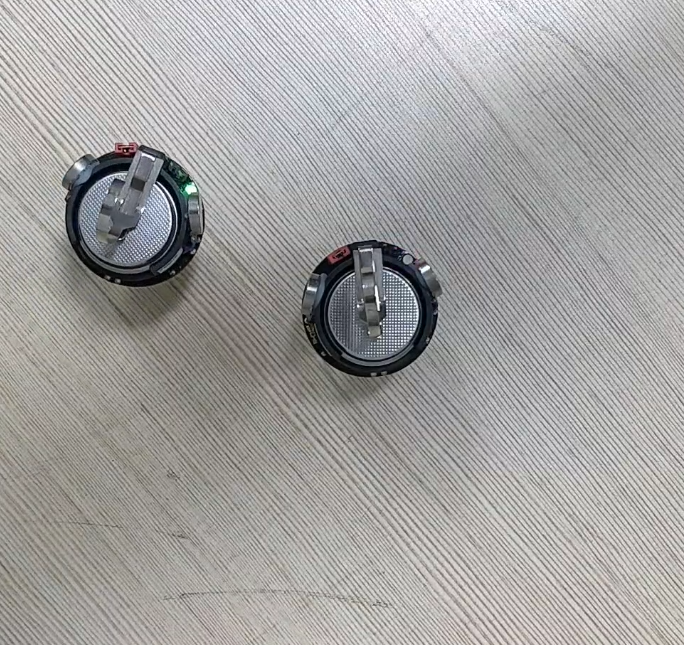
\includegraphics[width=2in]{orbit_after_escape}}
		\hspace{5cm}
		\caption{\href{https://youtu.be/X6dGCLT0ho8}{Escaping too close region of star by planet followed by orbiting}}
		\label{fig:shape_formation_demo}
	\end{figure}
	\end{column}
	\begin{column}{0.5\textwidth}
		\begin{figure}[H]
			\centering
			\fbox{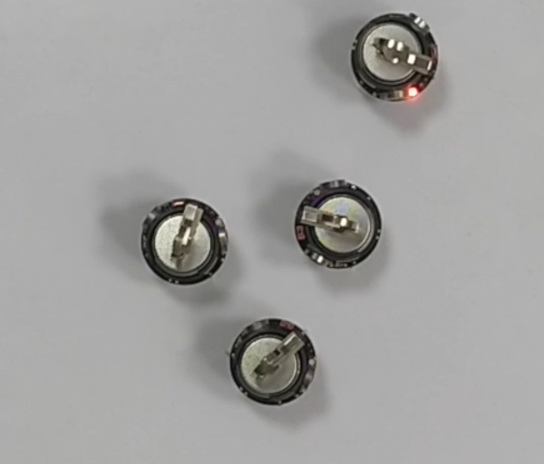
\includegraphics[width=2in]{orbiting_three_stars}}
			\hspace{5cm}
			\caption{\href{https://youtu.be/5aZm0Os9BPc}{Orbiting of planet around three stars using four communications to estimate minimum distance}}
			\label{fig:shape_formation_demo}
		\end{figure}
	\end{column}
	\end{columns}
\end{frame}
\section{Shape formation}
\begin{frame}
\only<1-2>{
	\frametitle{Shape formation}
	\only<1>{
		\textbf{Objective:} Distributed algorithm to generate a desired shape \cite{MR-AC-RN:2014}. 
	}
	\begin{columns}
		\begin{column}{0.5\textwidth}
			\begin{itemize}
				\only<1>{
					\item \textbf{Guides:} Index $0,1,2$ acts as reference for coordinate axis by continuously transmitting their index.
				}
				\only<2>{
					\item \textbf{Builders:} Index $3$ onwards for shape formation
					\item For forming a linear shape of width 2, the \textbf{shape matrix} would look like
					\hspace{5cm}
					\begin{align*}
					\label{eq:shape_matrix_linear}
					\begin{bmatrix}
					&Index & N_1 & DD_1 & N_2 & DD_2 &\\ 
					\cline{2-6}\\
					&3      & 1      & 1      & 2      & 1        &\\
					&4      & 2      & 1      & 3      & \sqrt{2} & \\
					&5      & 3      & 1      & 4      & 1        &\\
					&\cdots & \cdots & \cdots & \cdots & \cdots   &
					\end{bmatrix}
					\end{align*}
					\newline
					where,\\
					$N_i:$ Desired neigbour i\\ $DD_i$: Desired distance from neighbour i.
				}
			\end{itemize}
		\end{column}
		\begin{column}{0.5\textwidth}
			\only<1>{
				\begin{figure}
					\centering
					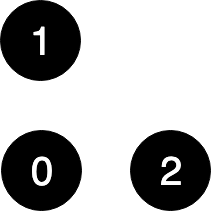
\includegraphics[scale=0.25]{shape_formation_process_guides}
				\end{figure}
			}
			\only<2->{
				\begin{figure}
					\centering
					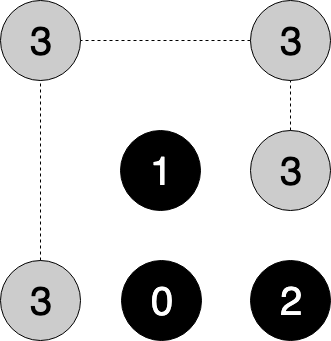
\includegraphics[scale=0.25]{shape_formation_process_1}
				\end{figure}
			}
			\only<2->{
				\begin{figure}
					\centering
					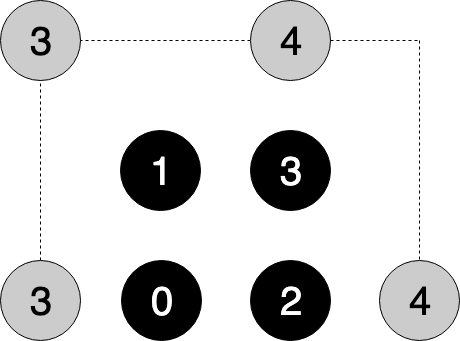
\includegraphics[scale=0.25]{shape_formation_process_2}
				\end{figure}
			}
		\end{column}
	\end{columns}
}
\only<3>{
	\frametitle{\small Flowchart}
	\begin{figure}
		\centering
		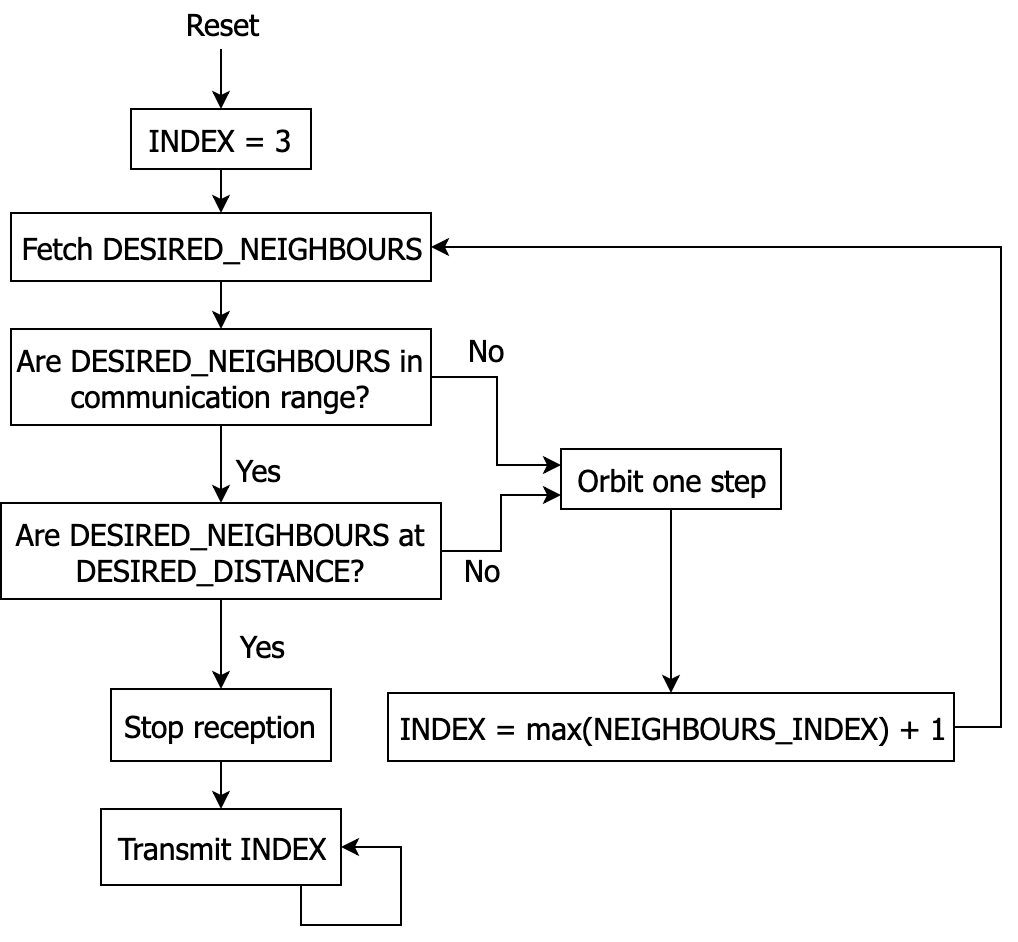
\includegraphics[scale=0.24]{shape_formation_ppt}
	\end{figure}
}
\only<4>{
	\begin{columns}[b]
		\begin{column}{0.5\textwidth}
			\begin{figure}
				\centering
				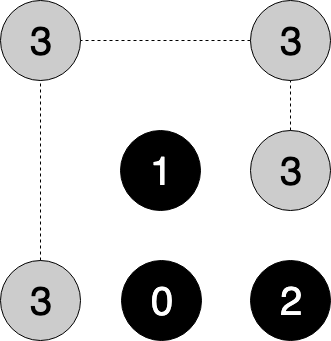
\includegraphics[scale=0.25]{shape_formation_process_1}
				\vspace{0.4cm}
				\caption{First builder}
			\end{figure}
		\end{column}
		\begin{column}{0.5\textwidth}
			\begin{figure}
				\centering
				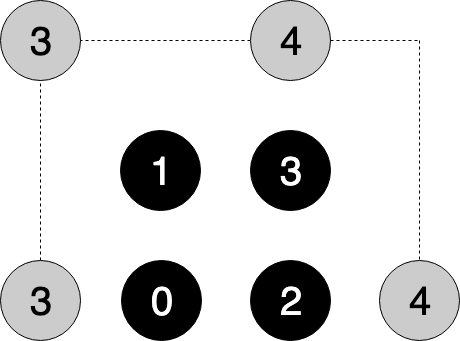
\includegraphics[scale=0.25]{shape_formation_process_2}
				\vspace{0.4cm}
				\caption{Second builder}
			\end{figure}
		\end{column}
	\end{columns}
}
\only<5>{
	\frametitle{Shape formation}
	\framesubtitle{Demonstration}
	\begin{figure}[H]
		\centering
		\fbox{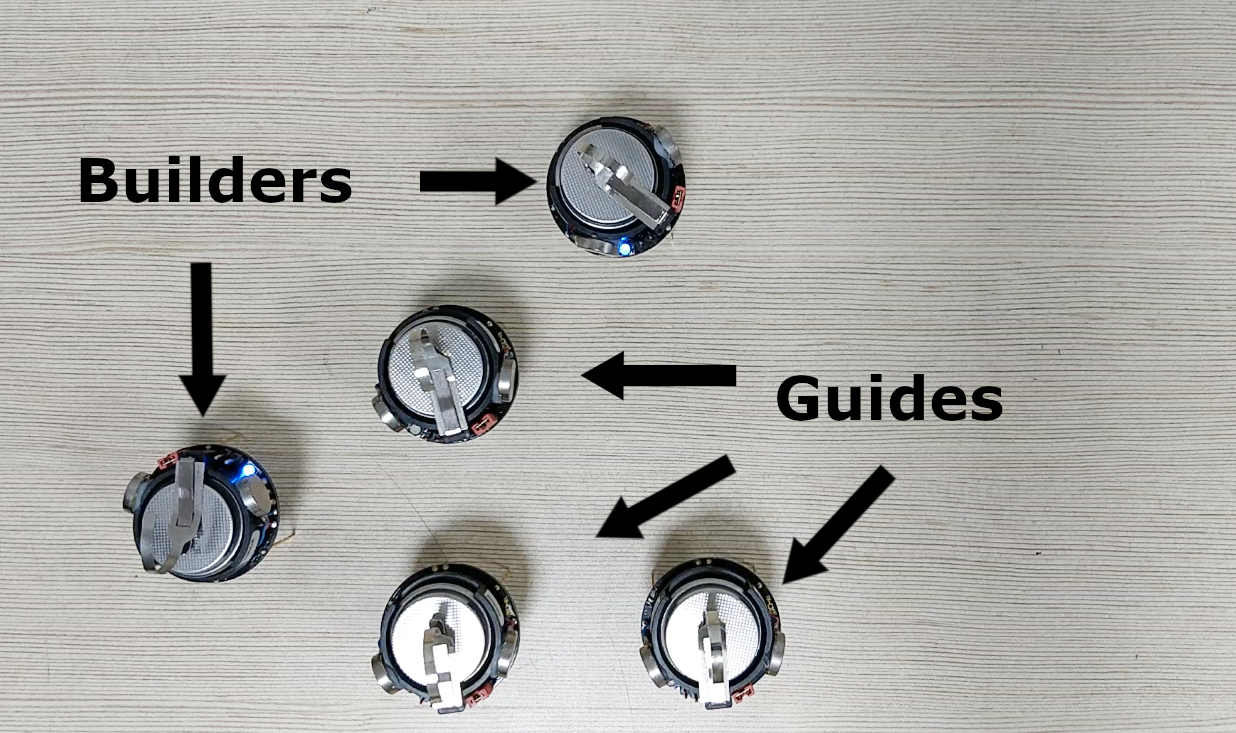
\includegraphics[width=3.5in]{shape_formation_demo}}
		\hspace{5cm}
		\caption{\href{https://youtu.be/SoDq9GQvNAE}{ Rectangle shape formation by Kilobots (l=3, b=2)}}
		\label{fig:shape_formation_demo}
	\end{figure}
}
\end{frame}

\end{document}